%update: Jan 14 fixed grammar according to prof notes
%update: Jan 13 add figure 4ways
%update: Jan 09-11 prof check
%update: finish writing Dec 30
%note: image 4waysprobe is not here

%\begin{savequote}[75mm] 
%We become what we behold. We shape our tools, and thereafter our tools shape us.
%\qauthor{Marshall McLuhan} 
%\end{savequote}

\chapter{Engineering of Probing Techniques inside TEM}

\newthought{We are not satisfied with the limited possibilities provided by TEM}, and we are eager to introduce more variables to the system because that is how we see dynamics in the real applications.
In the following subsections, I will firstly introduce how we cooperate chemicals, light, mechanical manipulations and electrical interactions within the microscopic experiment. 
Especially for the new optical fiber compatible TEM, where all the four factors could be merged, the inside and outside parts of the \emph{in situ} microscopic setup are described in detail. 
Finally I will take a look at the what the system can do and its short-comings. 

%before us, stm tem holder
\section{Introducing chemicals, electricity, strain into the microsocpe}

As I discussed in Chapter 1, \emph{in situ} microscopy does introduce parameters such as heat, cooling, gas, liquid, etc. to the system, but now I focus on how we delicately introduce these variables into the  microscope. In most cases, {\em in situ} microscopic experiments are performed by means of specially designed TEM holders, such as heating holder equipped with heating electrical wire or MEMS microheater. At the same time, some researchers made adaptions to the  microscope to introduce other variables. In my Ph.D. research, in addition to the electron beam, four more variables are introduced: chemicals (solid), mechanical probing, electrical contacting and optical access. \\

For electrical biasing, many TEM specimen holders are commercially available. Such holders provide a combination of TEM and Scanning Tunneling Microscopy(STM) techniques, which are employed simultaneously within one instrument. TEM characterization, STM imaging, introducing chemicals and electrical measurements- all become possible. The STM probe scanner has a very wide range of motions, from picometers to millimeters, which are employed either for a coarse adjustment of the sample orientation, or for a precise probe positioning. \\

Electrical contacts with nanoscaled interfaces can be realized under precise positioning of the movable probe to the desired spot, enabling simultaneous investigation of the specimen’s structural and electronic  properties with the optional strain or chemical transitions.\\

If the electrical biasing is realized through piezo probing, we can also utilize the probe for introducing chemical (solid on probe) and mechanical strain (without force value measurement\footnote{Introducing atomic force microscopy into TEM holder for mechanical measurements is another important {\em in situ} method without electrical biasing functions.}). \\

I briefly discussed the ways to input chemical, electrical biasing and mechanical factors in TEM. However, introducing  the other variable - light - to the system is challenging. Therefore I will discuss this part separately, which would be a very good reference for future research, in the next section. 

\section{Introducing light into the microscope}
\subsection{Previously}
Introducing the other factor - light - to the system, while at the same time maintaining the impact from other factors, is very tricky. Some researchers and companies tried to introduce light without probing. This means that no introduction of chemical changes, electricity and mechanics was achieved. We may first investigate how they introduce/collect light to/from the microscope. 
Table \ref{table2.1} compares the two possible ways to implement light into the system. 

\begin{table}[ht]
\centering 
\begin{tabular}{|c|c|} 
\hline 
by adaption to the microscope & by using special holder \\ [0.5ex] 
\hline 
light plane different from specimen & on same plane with specimen \\[1.5ex] 
require take off detector/aperture & a specially designed holder \\[1.5ex]
optics can be realized by lens on bench & only optical fiber\footnote{For the moment only optical fiber, but it is possible to have lens system inside the holder, please read Chapter 7 for more information.} \\[1.5ex]
complicated, high power, high cost & no adaption to TEM\\[1.5ex]
\hline
\end{tabular}
\caption{Two main ways to implement light into a TEM} 
\label{table2.1} 
\end{table}

As shown in the Table, by replacing an aperture or making a window for optical path the light path becomes tilted. The light goes through the microscope body at the different level from the specimen plane. In some cases, it is possible to replace a detector or an aperture by desired modules to provide more variables. As shown in Figure \ref{fig:2_1} under a certain angle, the light can reach the specimen. The system could be very complicated if the optics is realized through lens system on optical bench including light sources, lens system and options such as CCD camera, chopper and monochromator. The system can be very powerful if the optical system on table is well designed and precisely assembled. However, the pressure of time and high cost are expected to be very significant. \\

\begin{figure}  
\centering
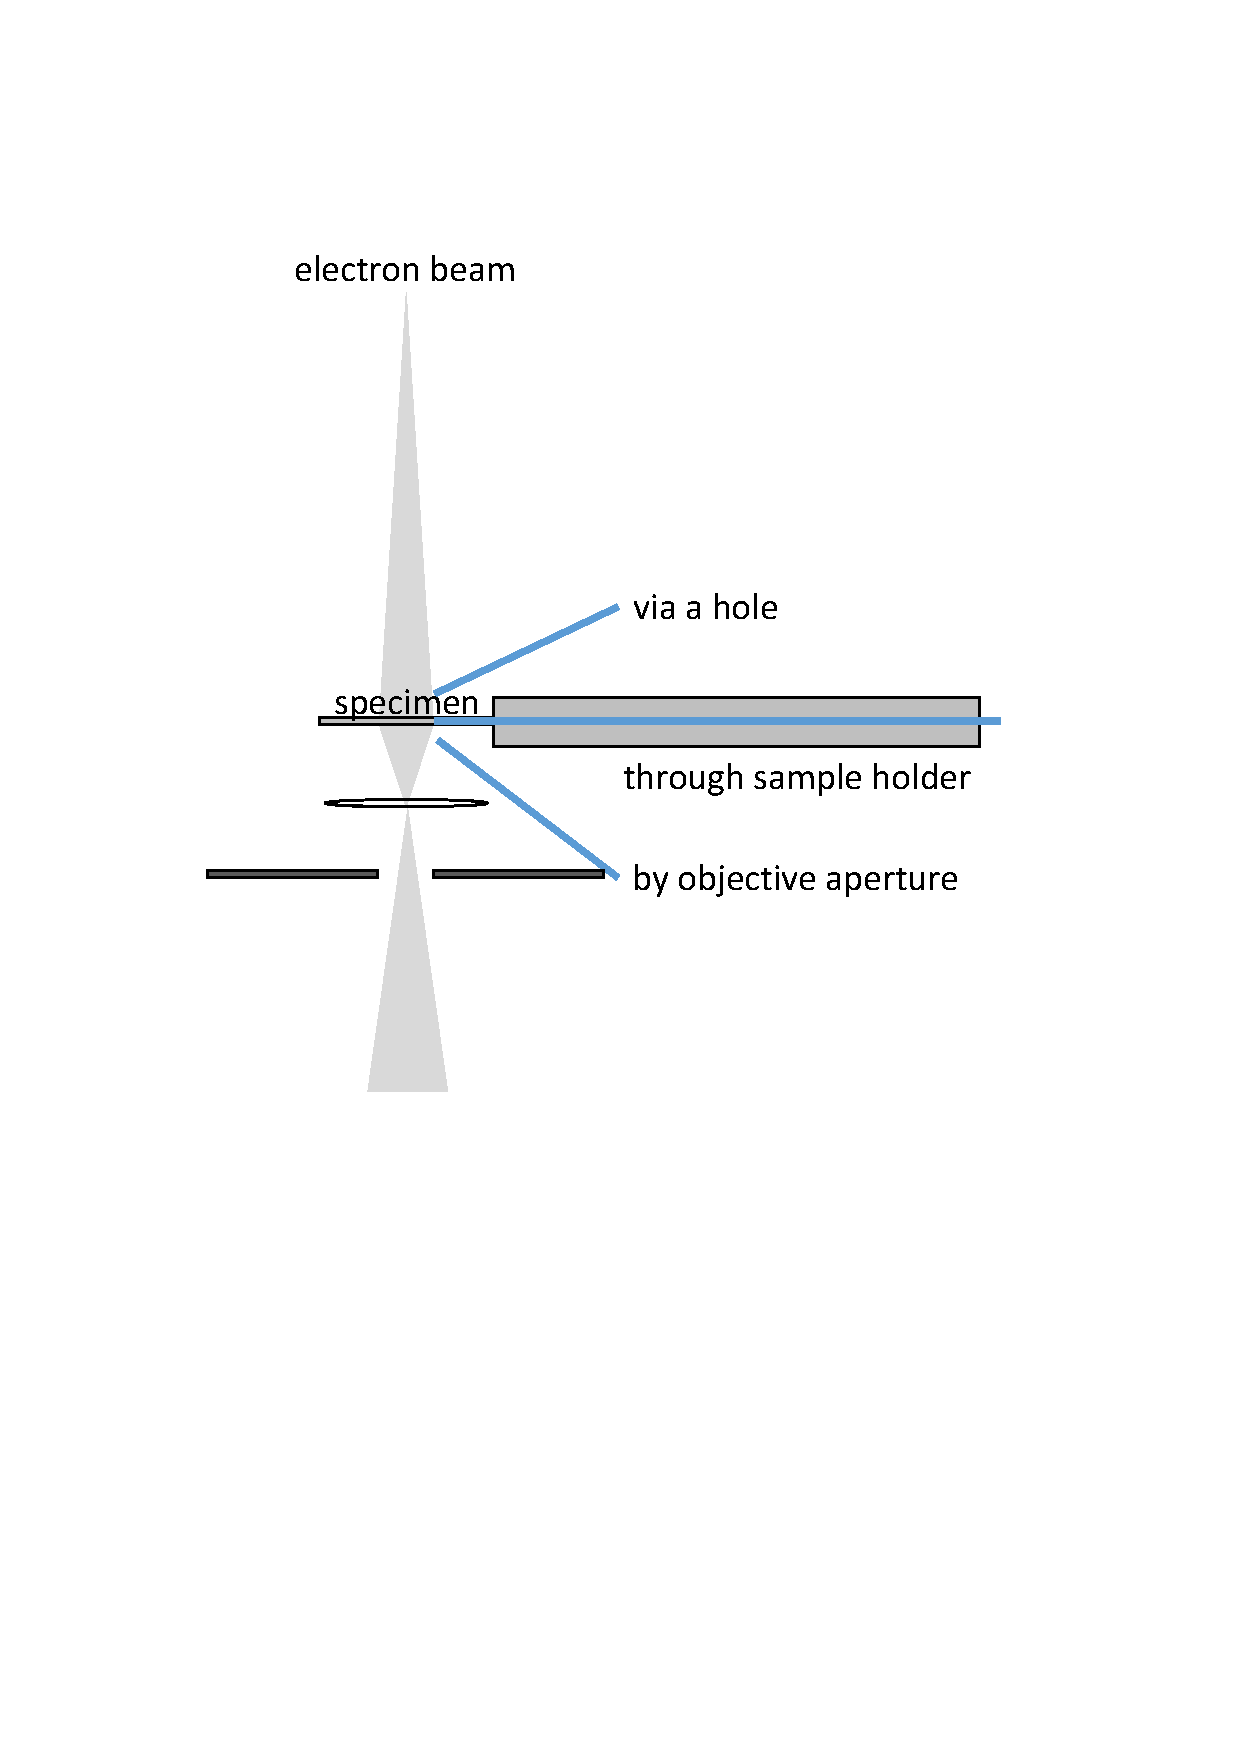
\includegraphics[width=320pt]{figures/figure2_1}
\caption[Putting light into TEM.]{How light is compatible to TEM.
\label{fig:2_1}}
\end{figure}

For a special optical holder, one way is to protrude an optical fiber through the holder, as shown in Figure \ref{fig:2_1}, the light will be shinning on the specimen at about 90 degrees to the direction of the electron beam. In most cases, the microscope is owned by many users for various applications, and therefore the approach of using special optical holder is more practical - it's quite unpractical to drill a hole in the microscope column and to install an optical bench on the microscope (given the fact that not every user will be happy with such operations). 

A few groups have tried to deliver light into TEM. \\

Muto et al. (Kyushu University) managed to install an optical fiber through a 2 mm hole at an angle of 45 degrees.\cite{Tanabe2002,Furumoto2013} They manufactured the prototype of TEM-CL system with the light collecting parts integrated on the holder, but no parabolic reflector was needed within the pole piece. The system is able to take cathodoluminescence(CL), X-ray emission spectroscopy and Electron Energy Loss Spectroscopy(EELS) at the same time, even under large angle sample tilts. The main disadvantage of the holder was a significant background level from the thermal glow of the electron gun and the CL signal from the optical fiber. Later, Muto et al.the same group and the staff from {\it Nanofactory Instruments} developed a prototype optical holder implemented with an optical fiber inserted through the holder, on the side of a specimen. The reflectors and optical fiber are placed away from the TEM optical axis. The light-collecting solid angle is approximately 1.3 strad, approximately 100 times larger than that of their first generation prototype. The sample is mounted at the end of the metal wire, which  position can be controlled to the focal point of the mirror by a piezo-driven manipulator. In years of 2012-2013, a few groups, including us, secured the optical holder (beta version) from {\it Nanofactory Instruments}. \\

One of the groups is in Brookhaven National Laboratory. Yimei Zhu et al. obtained the prototype optical holder from {\em Nanofactory} which allows for two optical fibers and several delicate mirrors to locate the light beam to the specimen. 
The multimodal optical nanoprobe allows scientists to perform standard experiments natural for TEM in addition to those involving optical excitation and measurements on the sample, including electrical measurements, STM and combinations of those. They emphasized the ability to simultaneously measure optical and electrical properties of the sample at the nanoscale.\cite{Zhu2012Multimodal}  The operations introduced are very similar to our case, but their serious problems were related to the calibration of light spot location, which had been realized by the adjustment of the tiny mirror screws; also, they were not able to confirm the location of light spot. Therefore the system was not that practical. \\

Minor et al. have implemented an {\it in situ} TEM monitoring technique to observe the crystallization of a-Si during high power pulsed laser irradiation by directly coupling laser into a TEM through a fiber-optics probe. By realizing a near-field scanning optical microscopy (NSOM) fiber probe scheme, this technique opens up a wide variety of new characterization possibilities.\cite{Xiang2012}

Kociak et al. of the Université Paris-Sud \cite{Zagonel2011} developed a STEM-CL system on a \textit{Nion} microscope which also uses an optical fiber as a light guide from the microscope column to the CCD camera outside the microscope. The light is collected by a specially designed mirror system of which the focus point is on the specimen. This CL-STEM imaging can be applied to obtaining luminescence spectra and imaging the structure simultaneously.\cite{Nagarajan2016Simultaneous}

In another group, Miller in Prof. Crozier's group in Arizona State University replaced the EDS detector (first version) or objective aperture (second version on FEI Titan microscope) with an optical fiber to shine a light onto chemicals to observe dynamics of photochemical reactions.\cite{Miller2012} 
But the problem was that they had not been sure about the location of the light spot, because they just could not observe it.

To conclude, by introducing light into TEM, these days the researchers are capable to observe dynamics of photochemical processes or thermo-effects, and to simultaneously obtain high resolution CL with EELS and Dark field imaging. As summarized in Table \ref{table2.2}, almost all groups used optical fibers for introducing light rather than lens system on bench, whereas most groups do not offer probing contacts capabilities. In my case (NIMS in Table), I would like to realize all these functions based on the redesigned optical holder. 

\begin{table}[ht]
\centering 
\begin{tabular}{|c|c|c|c|c|} 
\hline 
Institute & fiber & though & Probing contact & practical for\\ [0.5ex] 
\hline 
Nagoya U. & Yes & hole, holder direct & No & CL\\[1.5ex] 
BNL & Yes & holder by sides & Yes & N/A\\[1.5ex]
LBNL & Yes& holder direct & No & NSOM heating\\[1.5ex]
U. Paris-Sud & Yes & holder direct & No & CL-Map, NSOM\\[1.5ex]
ASU & Yes & detector/aperture & No & Photochem.\\[1.5ex]
NIMS & Yes & holder direct & Yes & all above\\
\hline
\end{tabular}
\caption{Comparison of the groups which introduced light to TEM} 
\label{table2.2} 
\end{table}

\subsection{Our holder adaption}
To choose between the fiber technology and the breadboard, it is necessary to define the objectives and a budget. 
A honeycomb core breadboard is a complex and powerful layout to customize optical input/output parameters with high precision. 

\begin{figure}  
\centering
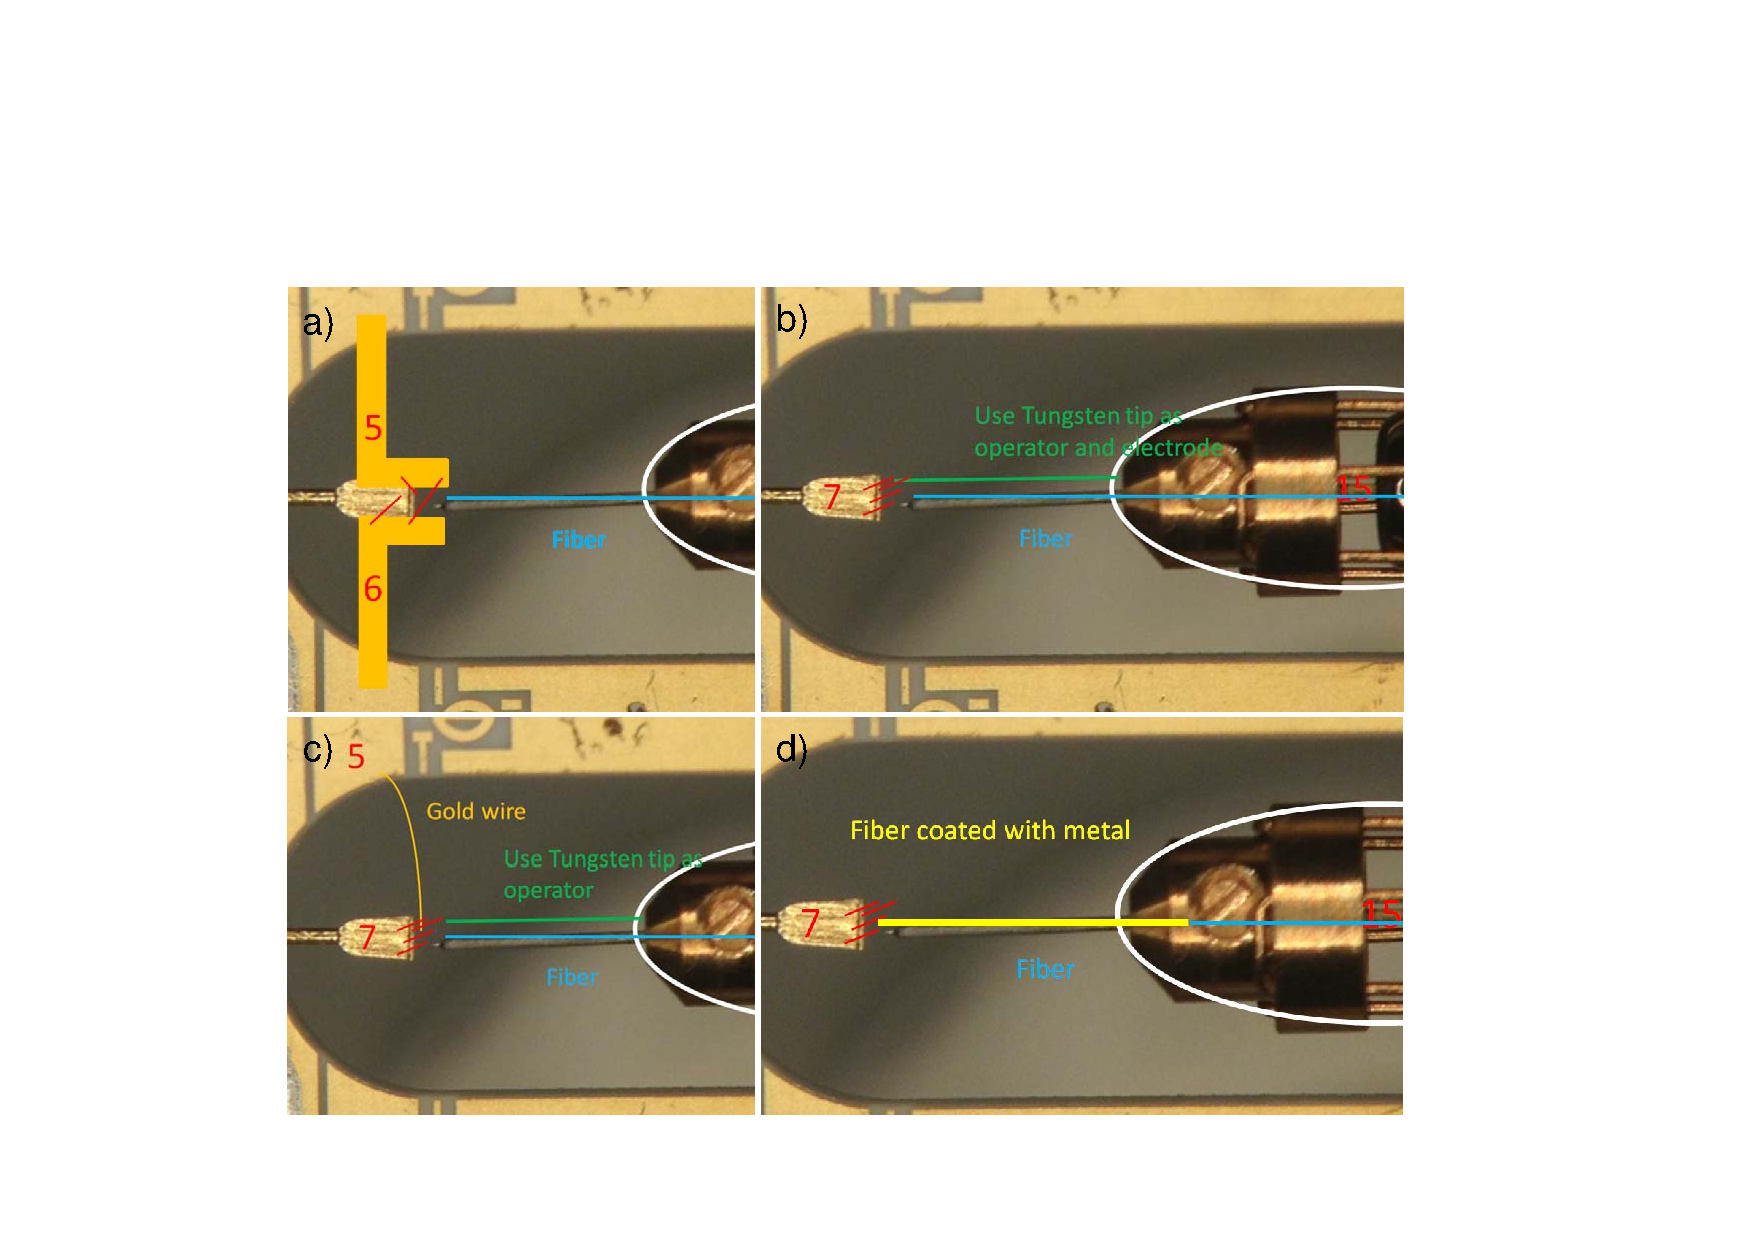
\includegraphics[width=320pt, angle=-90]{figures/figure2_4ways}
\caption[Proposed four ways of holder adaption]{Four schemes I proposed for introducing probing functions into the optical holder.
\label{fig:4ways}}
\end{figure}

However, building of an optical system on a honeycomb core breadboard could be costly. 
At least one optical window should be opened on the body of a microscope, so as to transmit an aligned laser beam into the chamber, and to collect optical signal from the chamber. 
In contrast, by using an optical fiber, a laser light could be easily introduced into the microscope without breaking the TEM column. 
The solution is to make a continuous hole through a special TEM holder, so as to insert an optical fiber in it. The former {\em Nanofactory Instruments AB} developed a holder for our Laboratory with a 250 micrometer pipeline. 

In our system, the microscope is not modified at all, and we integrate all the experimental dynamics through the specimen holder. 

The front frame of the special holder was placed into the 4 mm gap of the TEM pole
piece. And with the optical fiber inserted, the light connection between the TEM chamber and the outer space was realized. 

To develop the whole system based on the regarded general idea, the two issues for the setup should be of our prime concern. One issue is the inner TEM side – how to place the samples, how to design the fiber tip, how to operate and apply/test electrical signals on the samples. The other side is the outer TEM side – board development, space for light source and signal processing.  

\begin{figure}  
\centering
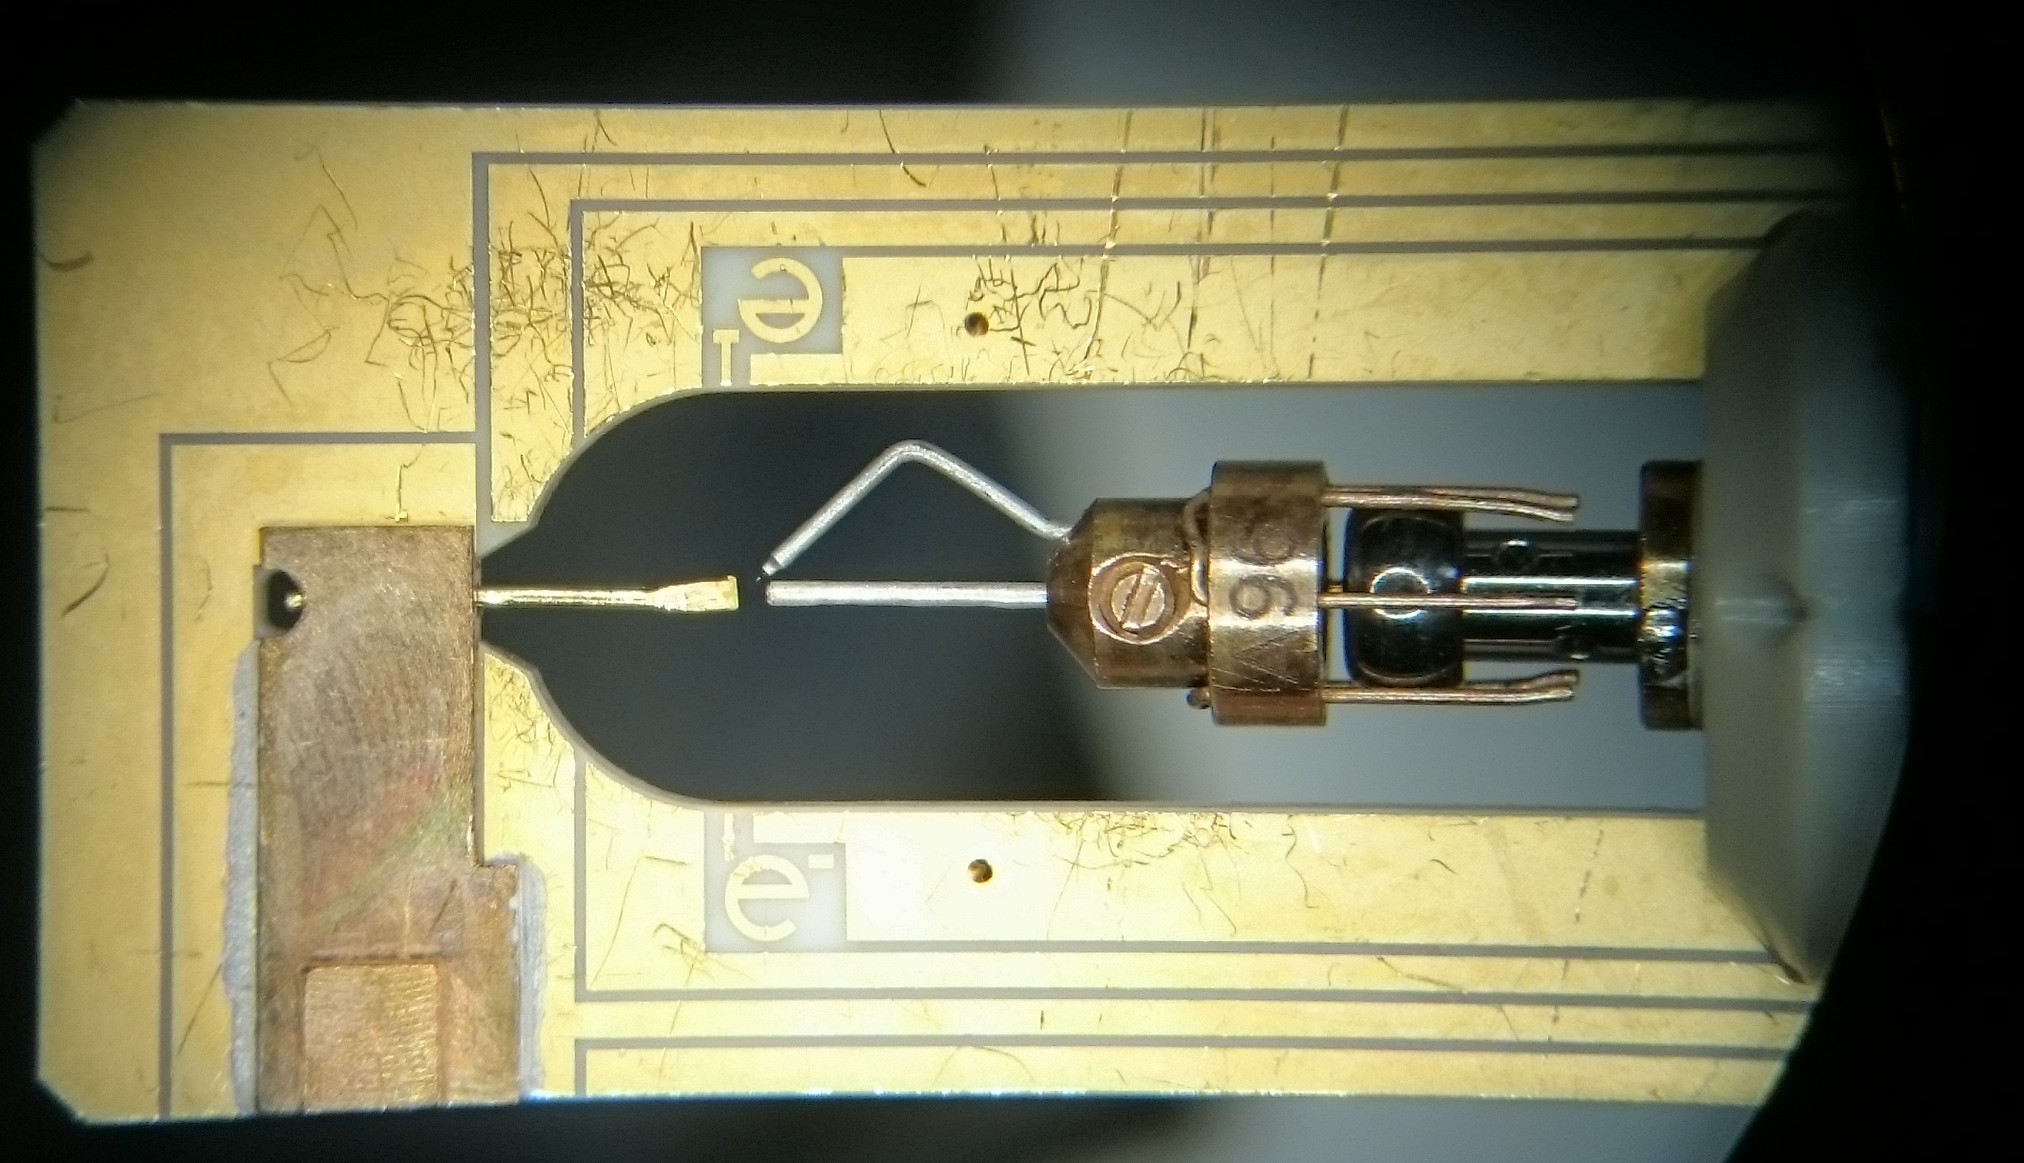
\includegraphics[width=\textwidth]{figures/figure2_holderframe}
\caption[Inner part of the holder]{The part of a holder inside the pole-piece of TEM to illustrate geometrical relationship between sample stage, probe, fiber and electron beam.
\label{fig:2_frame}}
\end{figure}

%%%%%%%%%%%%%%%%%%%%%%%%%%%%%%%%%%%%%%%%%%%%%%%%%%%%%%%%%%%%%%%%%%%%%%%%%%%%%
%%%%%%%%%%%%%%%%%%%%%%%%%%%%%%%%%%%%%%%%%%%%%%%%%%%%%%%%%%%%%%%%%%%%%%%%%%%%%%%
\textcolor{red}{
I proposed 4 ways to add electrical capabilities to the piezo-driven optical holder based on the \textit{Nanofactory} optical holder, as shown in Figure \ref{fig:4ways}. 
The are namely: \\
\begin{itemize}
	\item[a)] To build the separated arms on the frame and to place a sample across the arms (this can be very difficult) where it can be illuminated; 
	\item[b)] To drill a hole on the original cap, or to make a new hat with two holes and to install an additional probe; 
	\item[c)] Based on design b), one end of a gold wire can be placed on the electrical pad using a wire bonding machine, the other end of wire can be manipulated to make contact with the specimen, therefore, in total three electrodes become available; 
	\item[d)] To coat a conductive metal onto the surface (cross section is not coated) of the optical fiber (which is marked in yellow), the coating electrically joins the end (edge) of the fiber and the cap (an electrode); 
\end{itemize}
The possible ideas are not limited by these four ways. Combinations of a) and b), or a) and d) are also possible. By building arm(s), installing probe(s), bonding wire(s) and coating conducting layesr, electrical probing can enrich the functionality of the optical holder. 
}

%%%%%%%%%%%%%%%%%%%%%%%%%%%%%%%%%%%%%%%%%%%%%%%%%%%%%%%%%%%%%%%%%%%%%%%%%%

Considering the fact that attaching a probe onto the piezotube driven hat would enable more dynamic options available for our microscopy, I finally decided to drill a hole on side of the hat and to attach an additional metallic probe to it, while at the same time to coat a gold layer onto the fiber tip to reduce fiber charging during its exposure to an electron beam. 

\begin{figure}  
\centering
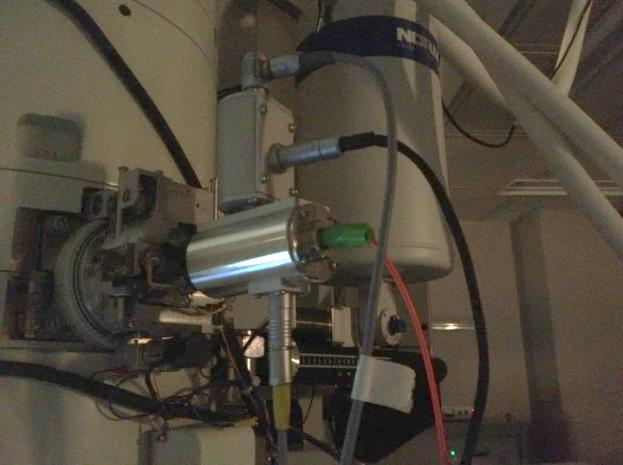
\includegraphics[width=\textwidth]{figures/figure2_holderbot}
\caption[Outside of holder]{The holder has several I/O ports for {\em in situ} mechanical, electrical and optical access.
\label{fig:2_bot}}
\end{figure}

For nanostructures, sampling is rather easy, the samples can be attached to the gold wire tip by touching, pressing, dipping or dropping, so that they could finally be exposed to an electron beam.
However, the optoelectronic {\em in situ} system could be more complex. The fiber tip inside TEM is clamped by a specialized cap which is driven by a XYZ-piezo controller. A tungsten probe for manipulation and electrical contacting is attached on the specialized cap manually. \\
Therefore, the sample is exposed to the electron beam and light, while at the same time it is controlled and connected by the stage (gold wire) and the tungsten probe. \\

For thicker samples, the specimens can be made by using a focused-ion beam (FIB) technique, or a half TEM grid may be used. 
The alignment of a sample, a fiber tip and the probe is quite important whereas rather difficult. If the fiber tip is far away from the sample, then the light will be divergent; this means that the power intensity of light could be reduced in progression. Since the tungsten probe will approach and connect the sample, the fiber tip should be as close as possible to the probe also. 

\begin{figure}
\centering
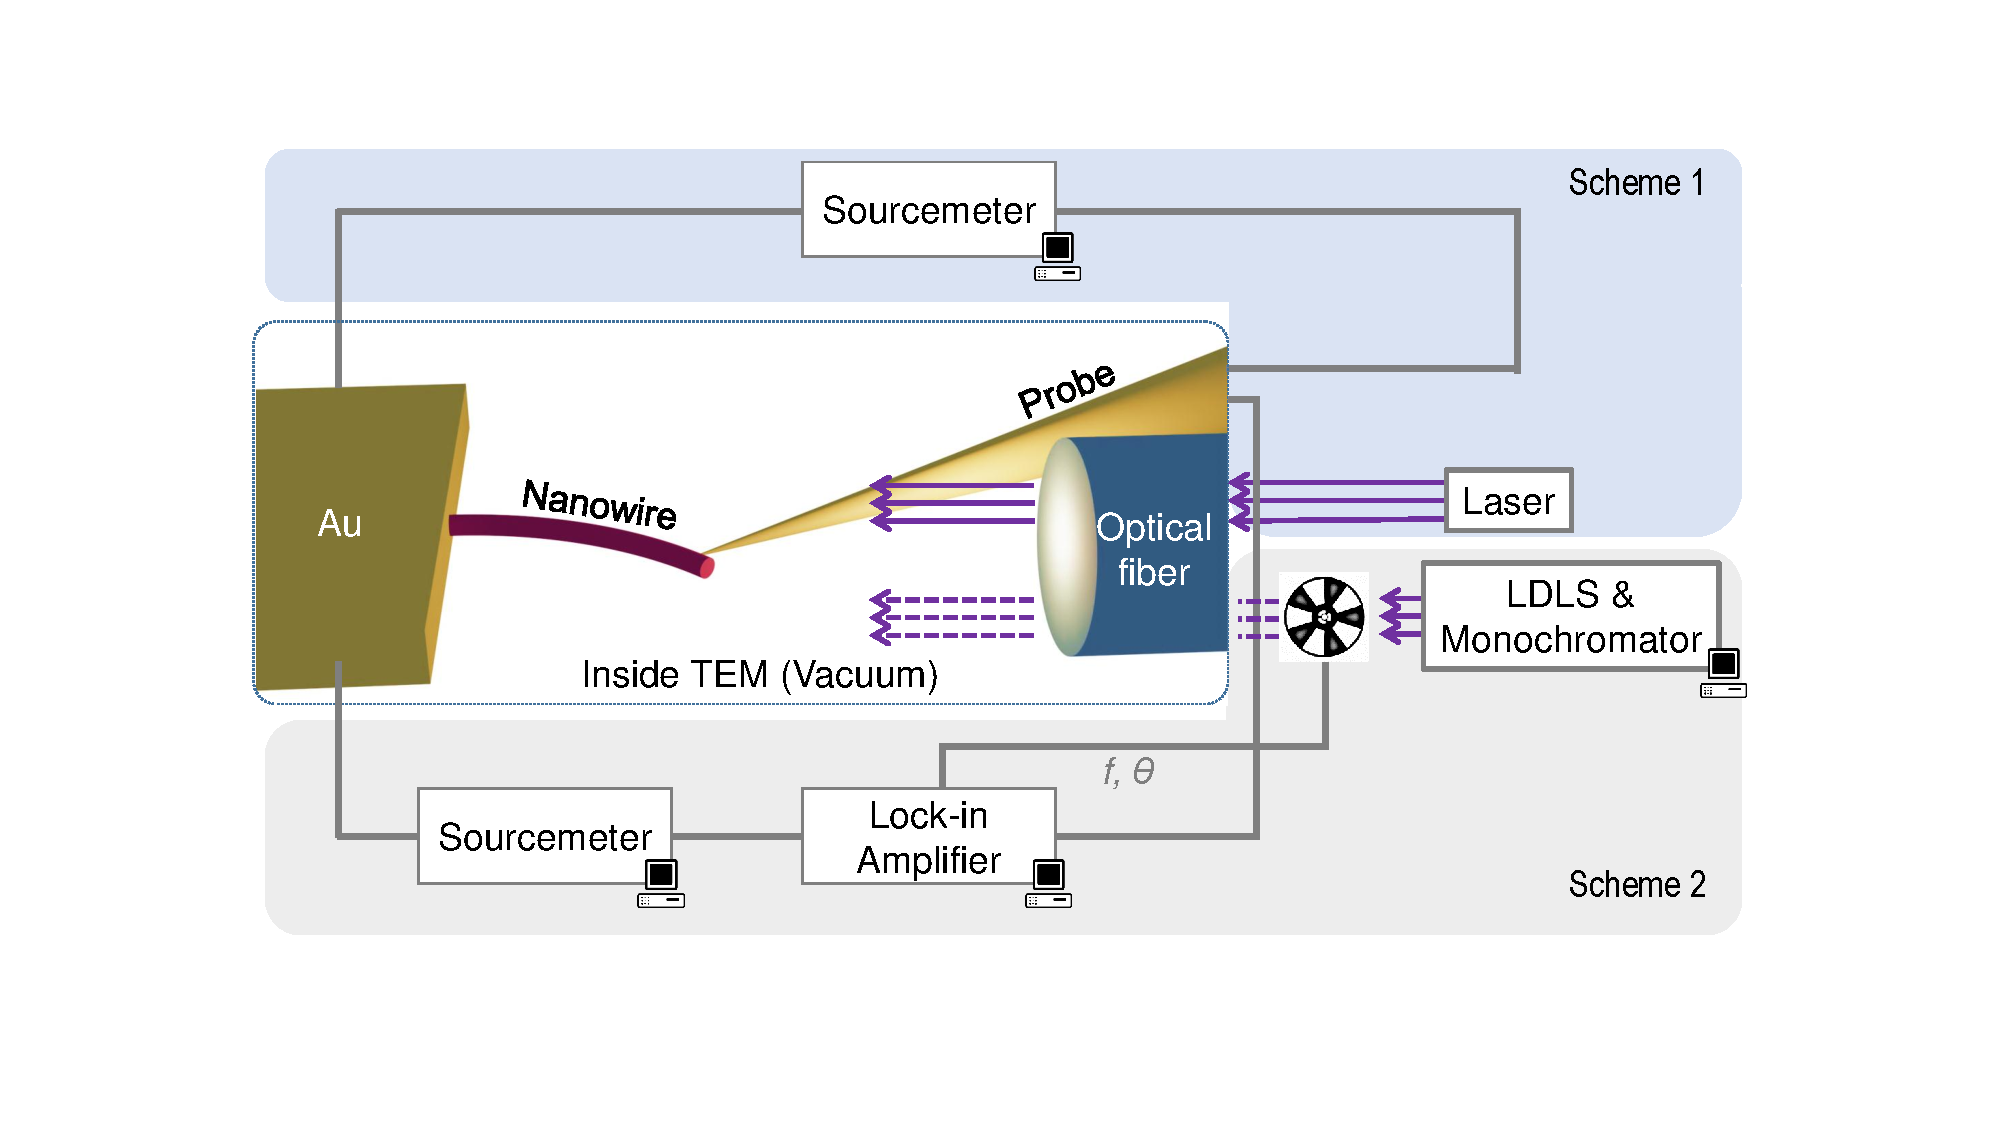
\includegraphics[width=\textwidth]{figures/figure6_1}
\caption[Optoelectronic {\em in situ} TEM scheme]{Optoelectronic {\em in situ} TEM scheme with two different light sources. }
\label{fig:6_1}
\end{figure}

In Figure \ref{fig:2_frame}, an image shows the geometrical relationship between the sample stage, probe, the fiber tip and electron beam. 

\subsection{Outer part of the microscope}
The individual coaxial electrical wiring through the holder for each contact gives pA level noises during the electrical measurements, allowing to measure low currents in Ohmic and non-Ohmic contact conditions. 

As shown in Figure \ref{fig:2_bot}, the holder has several ports for electrical, mechanical and optical signals to go in and out. 
The mechanical wire is at the downside, which is connected to the holder controller. 
The two electrical wires on top are connected to various electrical units depending on applications. 
At the bottom of the holder, optical fiber goes through and may serve as either a light source or a light detector, depending on application. 

A lock-in amplifier is used to extract a signal with an understandable carrier wave from a relatively noisy background. 
Because the light signal or photocurrent signal produced from a nanoscaled structure could be rather weak, detecting the signal against a bright noise could be accomplished using such amplifier. 
For example, in order to detect the photocurrents as a function of the wavelength of the incident beam one can apply a strong white light source, a chopper, a monochromator, a low-noise amperemeter and a lock-in amplifier. 
probe allow for measuring the electronic and optoelectronic responses. 

\begin{figure}  
\centering
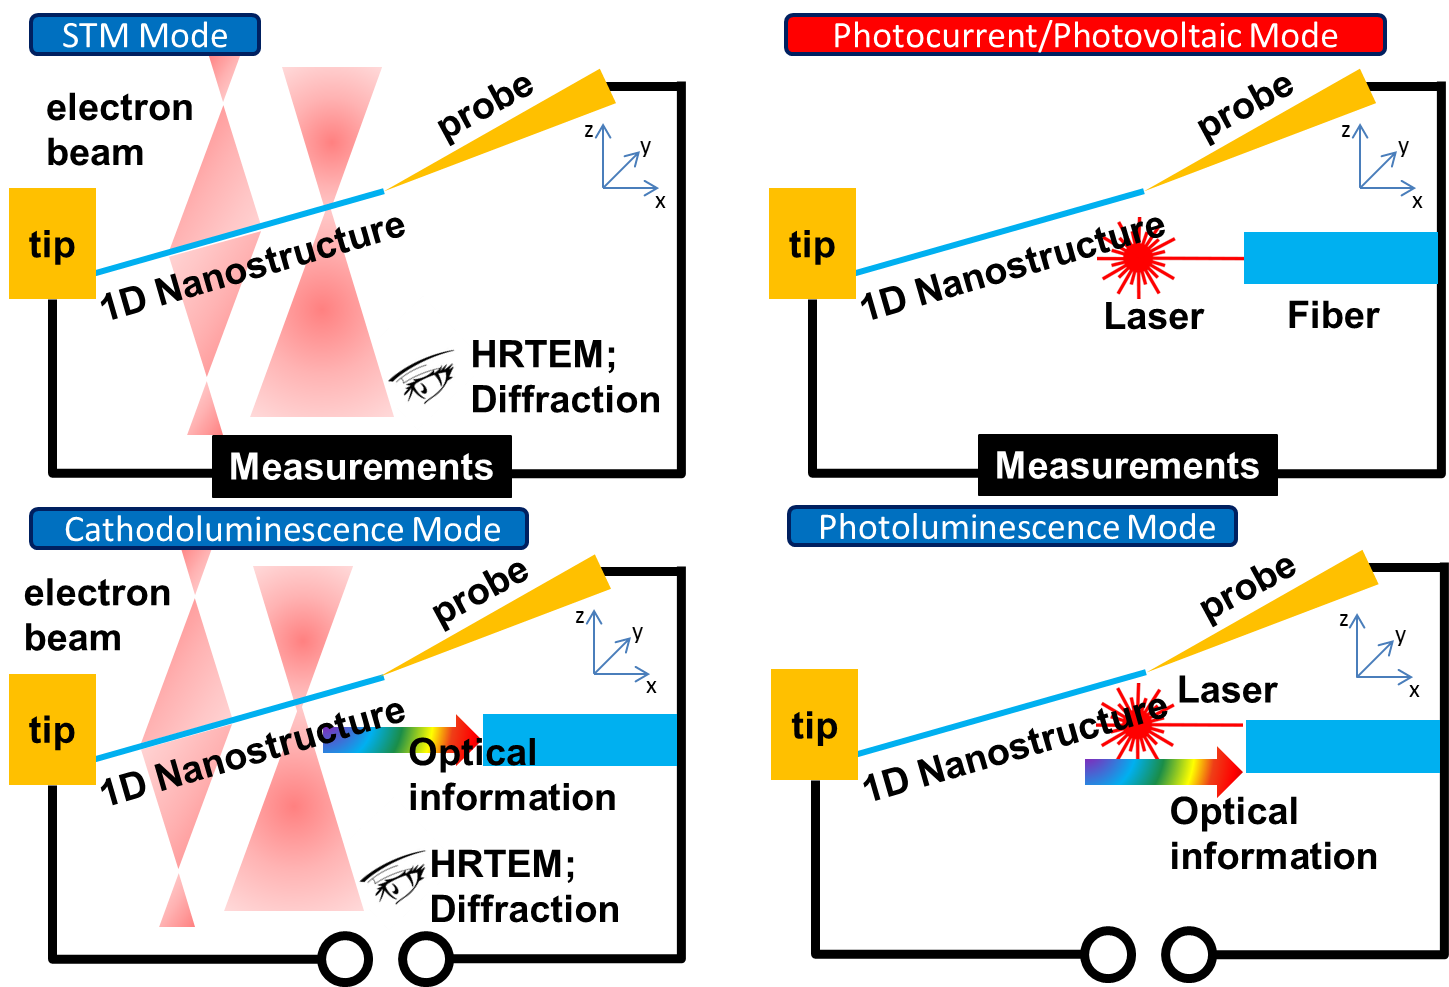
\includegraphics[width=\textwidth]{figures/figure2_fourmodes}
\caption[Four modes]{Four modes of light-compatible {\em in situ} TEM.
\label{fig:2_fourmodes}}
\end{figure}

Thus, the optical {\em in situ} TEM system was developed and optimized during the last few years. It is now multi-functional: 
as shown in Figure \ref{fig:6_1}: the white light source and monochromator are used together with the chopper and lock-in amplifier to measure the photocurrents as a function of wavelength. The laser diodes and wave signal generator are used together with the lock-in amplifier to measure photocurrents and photovoltages at a certain wavelength. 

The final system is fully compatible with both the laser light source and other light sources such as the Lazer-Driven Light Source (LDLS, Energetiq Technology, Inc.) used by us. Usually, the white light source is utilized in tandem with a monochromator. 

\section{Applications and limitations}
\subsection{Applications}
 The interface morphology, the contact area and orientation, the material crystallography - all of these factors can precisely be determined under high resolution microscopy, while a bias and a light applied onto the sample and 

Four modes were designed for different purposes. These modes are demonstrated in Figure \ref{fig:2_fourmodes}.\\

The first mode is the conventional STM-TEM mode, which allows for controlling, measuring and observing a nanostructure. This mode is used to manipulate with the structures and to observe the samples for detailed imaging, including high-resolution imaging and diffraction analysis. 
The system is also capable for applying chemical functions to the specimen for electrochemical experiments inside TEM. \\

The second mode is thought to be the most effective one. Photocurrent and photovoltage could be measured in addition to the conventional STM-TEM mode.
However, in order to get rid of the influence of electron beam on the sample, the electron beam should often be moved away from the sample when measuring.\\

The third mode is the CL mode. On the opposite way, the optical signal could be obtained through the fiber tip when one applies an electron beam to the structures. By collecting the optical signal from a specimen through the optical fiber, spatially resolved CL information can be gained and correlated to the crystallography information. Also electrical biasing or current flow are optional in this mode. \\

The fourth mode is the photoluminescence mode. The interference is only happened when two coherent waves are superimposed. The system is not yet available, but it is possible to establish. 

%On the opposite way, by collecting the optical signal from a specimen through the optical fiber, spatially resolved CL information can be gained and correlated to the crystallography information. 

\begin{figure}  
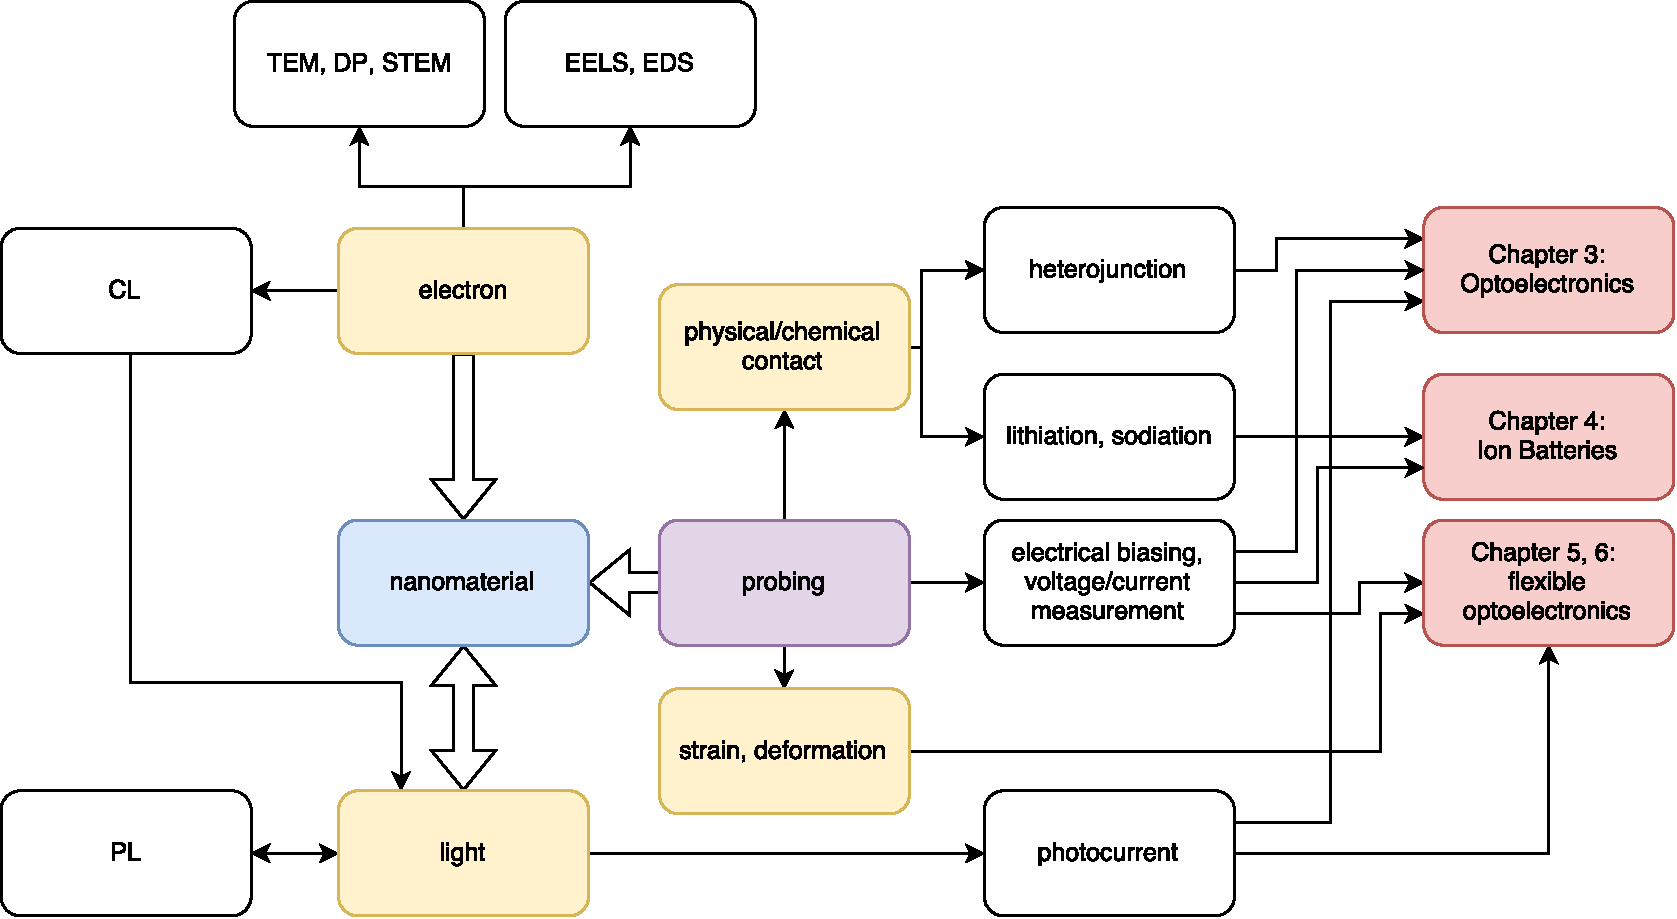
\includegraphics[width=\textwidth]{figures/figure2_apply}
\caption[Relationships between factors and applications.]{Relationships between factors and applications. Important dynamics is marked by yellow, some applications are marked by red, which will be detailed in other chapters.
\label{fig:2_apply}}
\end{figure}

In Figure \ref{fig:2_apply}, the relationships between each factors are presented. The applications of our light-compatible probing {\em in situ} TEM are not restricted to optoelectronics, flexible electronics/optoelectronics and lithium/sodium ion batteries, which are detailed discussed in Chapters 3-6. More fields, such as a research on CL, PL, photovoltaic and photochemistry applications are expected to be explored in the nearest future. 

\subsection{Limitations}
First, the system is based on TEM, therefore, all limitations of TEM are also applied to our system; that is, the sampling requirement is strict, the sampling efficiency is low, TEM imaging gives only 2D information, and electron beam may either damage the specimen, or interfere the experiment. 

Secondly, the incident beam is limited by the properties of the optical fiber and the light source. The optical fiber is not easy to replace, and is not recommended to do this frequently. 
Also, the optical fibers always have their own band pass windows for light, as well as maximum power limitations. 
For special requirements, for example, for UV/NIR light experiments, a proper UV/NIR light source and a proper UV/NIR fiber are required, the polarization of light needs a special optical fiber, etc. 

Thirdly, the mechanical force is not measurable. Even though I list mechanics as one factor of the system, the mechanical information is quite limited and is only related to the manipulation. In fact, we are able to see the strain (and then evaluate the force by simulations, at least qualitatively) based on deviations on 2D TEM images or diffraction patters, but we are not able to measure the detailed force values or strain/stress distributions directly. 

However well designed experiments and professional manipulations can eliminate, or, at least, reduce the burden of the limitations mentioned above. 
